\documentclass[journal]{IEEEtran}
\usepackage{graphicx,mathtools}

\begin{document}

\title{The Tor Network - Strengths and Weaknesses \\ \Large Computer Security 1 - CS5460 \\ \LaTeX{}}
\author{Jesse Victors \\ November 2013}

\maketitle

\section{Introduction}

The Tor network is a second-generation onion routing system that aims to provide anonymity, privacy, and Internet censorship protection to its users. Tour routes encrypted TCP traffic through a worldwide network of over four thousand relays run by volunteers across the world. Tor's encryption, authentication, and routing protocols are designed to make it infeasible for any adversary to identify an end user or reveal their traffic. Throughout its history, various organizations and governments have attempted to block, tap, or crack the Tor network. It was recently revealed that the US National Security Agency has attempted to penetrate the Tor network. Tor is also currently undergoing a transition from RSA-based to elliptic-curve-based TLS. In light of these attacks, Tor's popularity, and the protocol transition, a question that must be asked both by its users and by outsiders is: how secure is Tor? How does it work, what does it provide, and what are its weaknesses? In this paper, I attempt to address these questions.

\section{Design}

Tor provides an anonymity and privacy layer by relaying all end-user TCP traffic through a series of \textit{relays} on the Tor network. Typically this route consists of a carefully-constructed three-hop path known as a \textit{circuit}, which changes over time. These nodes in the circuit are referred to as \textit{entry guard}, \textit{middle router}, and the \textit{exit node}, respectively. Only the first node can determine the origin of TCP traffic through Tor, and only the exit node can examine the contents and its destination. Nodes in the middle are unable to determine either. No single node can determine the origin, the contents, and the destination of traffic through the network. Tor's architecture is designed to make it exceptionally difficult for a well-resourced adversary to uncover the identity of the end-user and their network activities, even if nodes are compromised.\cite{McCoy2008}

\subsection{Routing}

In traditional Internet connections, the client communicates directly with the server. In this model, an eavesdropper can often reveal both the identity of the end user and their activities. Direct encrypted connections do not hide IP headers, which expose source and destination addresses and the size of the payload. In the face of adversaries with sophisticated traffic analysis tools, such information can be very revealing for someone who wishes to hide their activities altogether.

Tor combats this by routing end user traffic through a randomized path through the network of relays. To construct this circuit, the Tor client software first queries a trusted directory server, which return a list of Tor nodes. This is illustrated in Figure 1.

\begin{figure}[htbp]
\centering
\begin{minipage}{8 cm}
    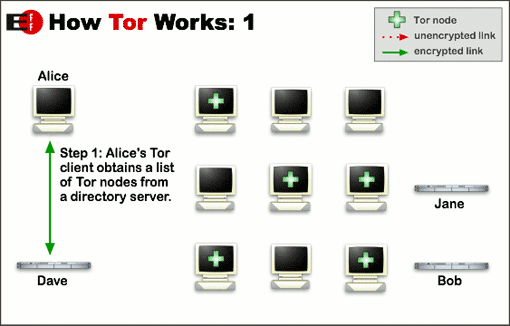
\includegraphics[width=80mm]{resources/circuit-building-1.png}
    \caption{The user's software first downloads a directory list of Tor relays. This information is later used to construct a circuit through the network.\cite{McCoy2008}\cite{TorOverview}}
\end{minipage}
\end{figure}

The second step involves choosing three nodes to use and carefully constructing an encrypted path between them. The circuit is extended one hop at a time such that no single relay ever knows the complete path. The client negotiates a separate set of encryption keys for each hop along the circuit to ensure that each hop cannot trace these connections as they pass through, as seen in Figure 2.

\begin{figure}[htbp]
\centering
\begin{minipage}{8 cm}
    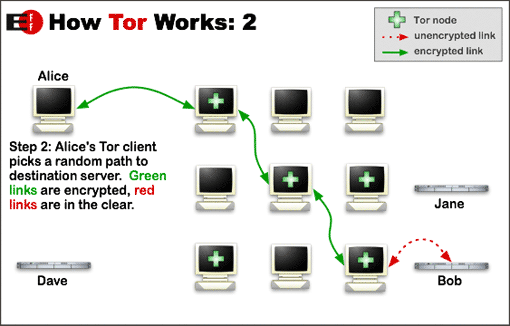
\includegraphics[width=80mm]{resources/circuit-building-2.png}
    \caption{A Tor circuit is incrementally constructed using layers of encryption. Each node has limited visibility, and no individual node knows the whole circuit.\cite{TorOverview}}
\end{minipage}
\end{figure}

Following the complete establishment of a circuit, the Tor client software then offers a Secure Sockets (SOCKS) interface which multiplexes TCP traffic through Tor. As each relay sees no more than one hop in the circuit, neither an eavesdropper nor a compromised relay can use traffic analysis to link the connection's source and destination. Tor further obfuscates user traffic by changing the circuit path every ten minutes,\cite{McCoy2008} as shown in Figure 3.

\begin{figure}[htbp]
\centering
\begin{minipage}{8 cm}
  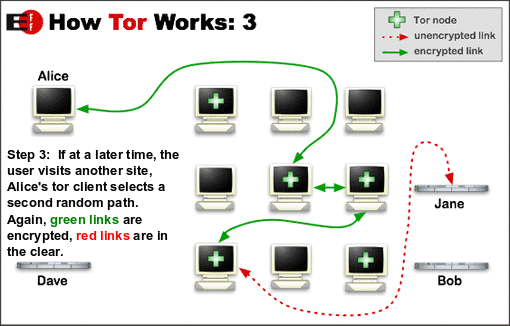
\includegraphics[width=80mm]{resources/circuit-building-3.png}
  \caption{A Tor circuit is changed periodically, essentially providing a new identity to the end user.\cite{TorOverview}}
\end{minipage}
\end{figure}

It should be noted that traffic exiting the Tor network is often (but not always) encrypted on its way to the source. An outsider is therefore faced with up to four layers of TLS encryption. Currently, Tor is one of the most secure tools to use against network surveillance, traffic analysis, and to bypassing information censorship.

\subsection{Encryption}

Encryption is a necessary component for privacy within the Tor network. Traffic passing between nodes must be secured from outsiders, and even compromised nodes must not be able to observe the traffic in cleartext. Privacy is also important for traffic outside the network; encrypted connections between the exit node and the target web server must also be achieved. Furthermore, two layers are needed: one for inside the network and one for outside it.

Within the network, nodes talk to each other via the Transport Security Layer (TLS) protocol. When a circuit is built, each pair of nodes within it must first come to an agreement over an encryption key and the specific cipher to use for encryption. There are several mechanisms by which this can be done, all of which use Diffie-Hellman (DH) for key exchange. The most common methods include: TLS\_RSA, which rely upon public and private keys generated with RSA; TLS\_DHE, ephemeral DH; TLS\_ECDH, DH based on elliptic curves, and TLS\_ECDHE, ephemeral elliptic curve DH. It should be noted that only TLS\_DHE and TLS\_ECDHE provide perfect forward secrecy, so it is no surprise that Tor exclusively prefers them. Once encryption keys and the specific cipher (as well as its mode) have been agreed upon, communication of traffic between two nodes can be encrypted and exchanged.

% http://security.stackexchange.com/questions/8343/what-key-exchange-mechanism-should-be-used-in-tls
% https://en.wikipedia.org/wiki/Comparison_of_TLS_implementations
% https://www.ipa.go.jp/security/rfc/RFC5246-ACJA.html
% 4134 -- 0x0039 TLS_DHE_RSA - the key exchange is an ephemeral Diffie-Hellman: the server dynamically generates a DH public key and sends it to the client; the server also signs what it sends. For DHE_RSA, the server public key must be of type RSA, and its certificate must be appropriate for signatures (the Key Usage extension, if present, must include the digitalSignature flag).
% 5566 -- 0xc013 TLS_ECDHE_RSA - the server sends a dynamically generated (ephemeral?) EC Diffie-Hellman key, and signs it with its own RSA key.

Tor users typically use the Tor Browser Bundle, (TBB) a custom build of Mozilla Firefox with a focus on security and pricacy. The TBB not only provides special handling of client-side scripts such as Javascript, but also offers the HTTPS Everywhere extension, which uses regular expressions to rewrite web requests into ones that use HTTPS. Thus, if the web server is capable of handling SSL or TLS connections, HTTP communications will be encrypted under them. Like any typical browser, the TBB negotiates with the web server for the cipher and keys required for SSL/TSL, except that this negotiation entirely occurs through the Tor circuit. As previously noted, this information, along with subsequent HTTP data, is encrypted between each node in the circuit. During transmission, each node in the circuit decrypts its layer in turn, until the final node (the exit) passes the data to the target server. The TLS/IP connections remain open, so the returned information likewise travels back up the circuit to the end user.

In September 2013, Robert Graham of Errata Security analyzed 22,920 incoming connections to his exit node and found that 89.9\% of the circuits agreed to use the Advanced Encryption Standard (AES) block cipher in cipher-block chaining (CBC) mode. This is the most common mode for AES, and allows for parallel decryption of the data blocks. The other 10.1\% of the circuits relied upon three rounds of the Data Encryption Standard (triple DES) cipher for encryption. Furthermore, 75.7\% of the circuits used elliptic-curve DH, with the remaining 22.3\% relying upon traditional RSA DH.\cite{Graham2013} Both protocols are discussed below.

\subsubsection{RSA}

RSA is an algorithm for public-key cryptography. Its security is based on the infeasibility of factoring the product of two large primes. RSA, like all other public-key cryptography algorithms, relies upon two keys: one public and the other private. The public key may be published and is used for encryption and for verifying digital signatures. The private key is used for decryption, the generation of digital signatures. Thus, through RSA, only the owner of the private key can decrypt incoming messages, and only they can digitally sign outbound messages. This makes RSA extremely powerful for both authenticity and privacy.

To generate the RSA keys, two distinct prime numbers of similar bit-length are chosen at random, \textit{p} and \textit{q}. \textit{n} is computed as the product of \textit{p} and \textit{q}, and it is used as the modulus for both the public and private keys. The bit-length of \textit{n} is the RSA key length. Then let $ \varphi(n) = \varphi(p)\varphi(q) = (p - 1)(q - 1) $ where $ \varphi $ is Euler's totient function, which counts the number of positive integers less than or equal to \textit{n} that are relatively prime to \textit{n}. Then \textit{e} is chosen such that \textit{e} and $ \varphi(n) $ are coprime. \textit{d} is also chosen such that it is the multiplicative inverse of e modulo $ \varphi(n) $. The RSA public key then consists of the modulus \textit{n} and the exponent \textit{e}. The private key likewise consists of \textit{n} and the exponent \textit{d}.

A message \textit{M} is encrypted by first blocks of length less than \textit{n} using an agreed-upon padding scheme. The ciphertext \textit{c} is then computed as $ m^e \bmod n $, which can be calculated quickly using the method of exponentiation by squaring. The owner of the private key can then recover the plaintext \textit{M} by computing $ c^d \bmod n $, and then reversing the padding scheme. The decryption process is often accelerated by optimizations such as the Chinese Remainder Theorem.

Furthermore, to sign a message, the owner of the private key first uses an agreed-upon hash function to compute a hash value of the message, raises it to the power of \textit{d} modulo \textit{n} and then sends that in conjuction with \textit{M}. The recipient, who only has access to the public keys, then raises the signature to the power of \textit{e} modulo \textit{n} and compares the result with his hash of the message using the same hash algorithm. If the two match, then he can prove the authenticity and integrity of the message. These two capabilities make RSA an extremely powerful tool for securing authenticity, integrity, and privacy of communication between two parties.

Tor version 2.3.x and previous rely upon TLS\_DHE for the key exchange mechanism. Per the TLS specification, the server generates a Diffie-Hellman public key and sends it to the client. The server also uses its RSA private key to sign everything that it sends to the client during the DH exchange. The client can then confirm the digital signature to verify the authenticity of the communication from the Tor relay.

\subsubsection{Elliptic-curve}

Elliptic Curve Cryptography (ECC) is an approach to public-key cryptography in which elliptic curves are used instead of RSA. In contrast to RSA, ECC relies upon the infeasiblity of finding the discrete logarithm of a random elliptic curve element with respect to a publicly known base point. This is known as the elliptic curve discrete logarithm problem, or ECDLP.

Elliptic curves over the real number system can be defined through the equation, $ y^2 = x^3 + ax + b $ where \textit{a} and \textit{b} are real numbers. This formula describes a plane curve through the Euclidean plane, although elliptic curves do exists in other spaces. However, current cryptographic purposes only work with elliptic curves within the context of the real number systems.

A smaller key size is one of the most significant benefits introduced by ECC. Current NIST recommendations state that a key size of 160 bits for ECC offers a similar level of security to 1024 bits of RSA/DH. Likewise, 224 bits for ECC is analogous to 2048 bits of RSA/DH. It should be noted that the required key sizes for ECC increases significantly slower than the key sizes for RSA and Diffie-Hellman increase at a much faster rate than the required key size for ECC. Thus ECC offers more security per increase in key size than for RSA. The smaller key size also directly correlates to an increase in computational efficiency; as the bit size increases, the speed difference between Diffie-Hellman and ECC grows superlinearly.\cite{CaseForECC}

Tor 2.4.x introduced TLS\_ECDHE, which uses an elliptic-curve variant of the Diffie-Hellman key exchange. Like TLS\_DHE, the server uses its RSA key to digitally signs communication to the client. The TLS\_ECDHE protocol is believed to be more secure than TLS\_DHE.

\subsubsection{Symmetric-key}

% http://www.isg.rhul.ac.uk/tls/
% https://community.qualys.com/blogs/securitylabs/2013/03/19/rc4-in-tls-is-broken-now-what

Once the SSL/TLS handshake completes, both parties use the generated session key and turn to symmetric-key encryption for hiding of data.

Data Encryption Standard (DES) is a block cipher introduced in 1977 by IBM. It was considered insecure in 1998 when the DES Challenges demonstrated that it was feasible to brute-force DES ciphertexts in a matter of hours using custom hardware. This weakness was partially mitigated by the introduction of triple DES (3DES) in the same year, where three rounds of DES were performed using three separate 56-bit keys. However, 3DES was found to be susceptible to meet-in-the-middle, chosen-plaintext, and known-plaintext attacks, so despite using a 168-bit key, 3DES only provides 80 bits of security.\cite{NIST2007} 3DES is still used on the web and by older Microsoft products, but has been largely superseded by other algorithms.

Advanced Encryption Standard (AES) is a block cipher introduced in 2001. It supersedes 3DES, and is now used extensively worldwide. AES became the recommended cipher for protecting classified documents for the US government in 2003, and side-channel attacks on specific implementations were the only known vulnerabilities up until mid 2009. To date, the most successful public attacks require $ 2^126.1 $ operations to recover a 128-bit key,\cite{Nikolic2009} and related-key attacks can break AES-192 and AES-256 in $ 2^176 $ and $ 2^99.5 $ operations,\cite{Bogdanov2011} respectively.

RC4 is a stream cipher invented in 1987 and sunsequently leaked in 1994. The RC4 algorithm is simple and extremely fast in software, and is now the most widely used software stream cipher, most notably in protocols such as TLS and WEP. Although it is popular, a number of practical attacks and weaknesses have been demonstrated against its Key Scheduling Algorithm and PRNG that call into question RC4's security. In November 2013, Microsoft recommended disabling RC4 from TLS wherever possible.

Robert Graham's analysis of the incoming handshakes to his exit node revealed that almost 90\% of the circuits agreed on the AES cipher, while the remainder used 3DES. For communication to web servers, RC4 remained the most popular algorithm.

\section{Attacks and Defenses}

Attacks from adversaries against Tor can be classified into several categories: attack on the user, attacks on their computer, attacks on the Tor network itself, attacks on the exit's connection across the Internet, and attacks on the server. Tor's developers have implemented or recommended various defenses against common attacks on each of these layers.

\subsection{Weaknesses introduced by the user}

Users on Tor must take precautions when using Tor. Although Tor's onion routing provides privacy and anonymity to their traffic, users can identify themselves by revealing their real name or information about where they are. If they build an electronic trail that can be used to deanonymize them, the use of Tor is rendered useless by their carelessness.

(going to expand this a bit more)

\subsection{Attacks on user's computer}

Tor users can also be revealed or have their privacy compromised by their own workstations. If their computer contains spyware, backdoors, or other malicious software that can be used to identify them or their traffic, then a user may be tricked into believing that they are anonymous when in fact they are not.

(going to expand this a bit more, discuss Javascript vs NoScript, cross-site scripting attacks, TBB defenses)

\subsection{Attacks on the Tor network}

The relay chosen for the first hop in the circuit has knowledge of the user's IP address, can thus deanonymize them in that respect. Although this first relay does not know the rest of the circuit and cannot deduce the final traffic exiting Tor, the knowledge of the user's IP can be problematic if the relay is operated by an attacker. With this information, an adversary would be able to trace users or deny them entry into the Tor network.

Tor combats this through \textit{entry guards}. The Tor client software chooses three relays out of the pool and then exclusively uses one of these chosen relays as the first hop of the circuit. This protects the end user against the \"predecessor attack\", wherein the attacker can preform end-to-end correlation and deanonymize the user if compromised nodes are chosen for the first and last hop in the circuit,\cite{Wright2004} and they make it more difficult for an attacker to add some relays to the Tor network and immediately begin tracing users. As of the time of this writing, there are 4,737 relays on the Tor network, so the chances of a client including a compromised node in its selection pool is 4,737 choose three without replacement, or 0.06334\%.

Tor is susceptible to timing attacks. To achieve its low-latency objective, Tor does not explicitly re-order or delay packets within the network.\cite{McCoy2008} Therefore, if an adversary controls both the first hop and the final hop in the Tor circuit then they can use statistical timing tests to become reasonably confident in identifying the activities of the end-user. %For example, they could observe 198.51.100.37 connecting to their first node

(going to expand this a bit more, add some citations)

\subsection{Compromising the exit node}

Exit nodes are valuable on the Tor network due to their necessity for the final hop of the circuit and because they are rarer than traditional relays. Exit node operators typically have to deal with ISP complaints for any nefarious Internet activities performed by the users at the other end of the circuit. Although these complaints can be largely combated by implementing a reduced exit policy, there are 912 exit notes at the time of this writing, 19.74\% of the total 4,737 relays on the Tor network. It is entirely possible than an adversay could control an exit node, giving them insight into the traffic leaving Tor. If the traffic is encrypted, the exit node could still see the DNS lookup and HTTP headers. If encryption is not implemented, all traffic would thus be available for inspection.

In September 2007, Swedish security consultant Dan Egerstad operated five exit nodes and monitored their traffic. Over the course of his experiment, he obtained the usernames and passwords for over 100 email accounts, read the correspondence from embassies in Australia, Japan, Iran, India, and Russia, along with communication between dignitaries including the Indian ambassador to China, various politicians in Hong Kong, workers in the Dalai Lama's liaison office, and several human-rights groups in Hong Kong. He also obtained sensitive spreadsheets and documents about military and political activities. Egerstad's analysis further revealed that approximately 95\% of the traffic flowing over his nodes was not encrypted.\cite{Wired2007}

An adversary could operate one or more exit nodes, as Egerstad did, or they could wiretap the exit's traffic and gain access to the traffic that way, perhaps without the knowledge of the exit operator. While the exit has no knowledge of the entire circuit and thus cannot deduce the origin of the traffic, the unencrypted traffic can be quite revealing and problematic, as Egerstad demonstrated. The primary way that Tor combats this through encryption. The Tor Browser Bundle comes with the HTTPS Everywhere, which prefers the use of HTTPS when connecting to web servers. Most email servers also support SSL/TLS, and users can also manually encrypt their documents or emails using PGP. Although Tor has no way of enforcing this final layer of encryption, it highly recommends it and places notices about this on many places on its website.

\subsection{Attacks on the web server}

The web server can also be a point of failure for the privacy and anonymity of the end user.

(going to expand this a bit more. Does the web server support SSL/TLS? The adversary could fake masquerade as the server)

\section{Adversaries}

% https://blog.torproject.org/blog/improving-tors-anonymity-changing-guard-parameters

%It was recently revealed that the National Security Administration (NSA) has been targeting Tor, albeit with marginal success in breaking the anonymity and privacy of its users. However, in early October, the FBI successfully identified and arrested the owner of the Silk Road, a black market operating as a hidden service within the Tor network, and seized the service.

(going to expand this a bit more, discuss NSA, FBI, Silk Road, China, etc)

\section{Analysis}

(going to expand this a bit more and devote the couple pages to this section. I've got IEEE citations like \cite{Xin2009}, \cite{Ling2011}, and \cite{Ling2012} that should be very helpful in demonstrating some weaknesses of Tor

\section{Conclusion}

(obviously I need this. Summarize design, attacks, defenses, analysis, reviews in the literature, and then provide my opinion about the future)

% -----------------------------------------------------------------------------

% https://en.wikibooks.org/wiki/LaTeX/Bibliography_Management
\begin{thebibliography}{9}

% http://freehaven.net/anonbib/#Wright:2004
\bibitem{Wright2004}
  Matthew Wright, Micah Adler, Brian Neil Levine, and Clay Shields
  \emph{The Predecessor Attack: An Analysis of a Threat to Anonymous Communications Systems}.
  ACM Transactions on Information and System Security (TISSEC) 4(7), November 2004, pages 489-522

% http://ieeexplore.ieee.org/stamp/stamp.jsp?tp=&arnumber=5636000&tag=1
\bibitem{Chaabane2007}
  Abdelberi Chaabane, Pere Manils, Mohamed Ali Kaafar
  \emph{Digging into Anonymous Traffic: a deep analysis of the Tor anonymizing network}.
  IEEE, 2010

% http://www.wired.com/politics/security/news/2007/09/embassy_hacks
% http://www.wired.com/threatlevel/2007/08/embassy-e-mail/
\bibitem{Wired2007}
  Kim Zetter
  \emph{Rogue Nodes Turn Tor Anonymizer Into Eavesdropper's Paradise}
  Wired, 2007

% http://csrc.nist.gov/publications/nistpubs/800-57/sp800-57-Part1-revised2_Mar08-2007.pdf
\bibitem{NIST2007}
  Elaine Barker, William Barker, William Burr, William Polk, and Miles Smid
  \emph{Recommendation for Key Management, Part 1: General (Revised)}
  National Institute of Standards and Technology, March 2007

% http://delivery.acm.org/10.1145/1320000/1314336/p11-bauer.pdf?ip=129.123.212.2&id=1314336&acc=ACTIVE%20SERVICE&key=C2716FEBFA981EF14CED21A2601DAAECFD63F9AFA4F38248&CFID=375634674&CFTOKEN=21383502&__acm__=1383519744_1cd525050cafbe9ffe083b269ff783d9
\bibitem{Bauer2007}
  Kevin Bauer, Damon McCoy, Dirk Grunwald, Tadayoshi Kohno, Douglas Sicker
  \emph{Low-resource routing attacks against tor}.
  ACM, 2007

% http://homes.cs.washington.edu/~yoshi/papers/Tor/PETS2008_37.pdf
\bibitem{McCoy2008}
  Damon McCoy, Kevin Bauer, Dirk Grunwald, Tadayoshi Kohno, Douglas Sicker,
  \emph{Shining Light in Dark Places: Understanding the Tor Network}.
  Department of Computer Science and Engineering,
  University of Washington, Seattle, WA 98195-2969,
  2008.

% http://link.springer.com/chapter/10.1007%2F978-3-642-03356-8_14
\bibitem{Nikolic2009}
  Nikolić, Ivica
  \emph{Distinguisher and Related-Key Attack on the Full AES-256}
  Advances in Cryptology, 2009

% http://ieeexplore.ieee.org/stamp/stamp.jsp?tp=&arnumber=4797313
\bibitem{Xin2009}
  Liu Xin, Wang Neng
  \emph{Design Improvement for Tor Against Low-Cost Traffic Attack and Low-Resource Routing Attack}
  2009 International Conference on Communications and Mobile Computing

% http://www.nsa.gov/business/programs/elliptic_curve.shtml
\bibitem{CaseForECC}
  National Security Agency
  \emph{The Case for Elliptic Curve Cryptography}.
  NSA, 2009

% https://research.microsoft.com/en-us/projects/cryptanalysis/aesbc.pdf
\bibitem{Bogdanov2011}
  Andrey Bogdanov, Dmitry Khovratovich, and Christian Rechberger
  \emph{Biclique Cryptanalysis of the Full AES}
  Microsoft Research Redmond, 2011

% http://ieeexplore.ieee.org/xpls/abs_all.jsp?arnumber=5962653
\bibitem{Ling2011}
  Zhen Ling
  \emph{Equal-Sized Cells Mean Equal-Sized Packets in Tor?}
  IEE International Conference on Communications, 2011

% http://ac.els-cdn.com/S1389128612003799/1-s2.0-S1389128612003799-main.pdf?_tid=c6751d5e-5009-11e3-9ab2-00000aab0f26&acdnat=1384749046_78b8af8ba2cb2c0a2672840e0c7c5da1
\bibitem{Ling2012}
  Zhen Ling, Junzhou Luo, Wei Yu, Xinwen Fuc, Weijia Jia, Wei Zhao
  \emph{Protocol-level attacks against Tor}
  Computer Networks, 2012

% http://blog.erratasec.com/2013/09/tor-is-still-dhe-1024-nsa-crackable.html
% http://thehackernews.com/2013/09/NSA-can-crack-TOR-Encryptio-Snowden-files-.html
\bibitem{Graham2013}
  Robert Graham
  \emph{Tor is still DHE 1024 (NSA crackable)}.
  Errata Security, 2013

% https://www.torproject.org/about/overview.html.en
\bibitem{TorOverview}
  Overview of Tor

% https://www.torproject.org/docs/faq.html.en
\bibitem{TorFAQ}
  Tor FAQ

\end{thebibliography}

\end{document}
